\section{Evaluation}\label{sec:evaluation}

In this section we present a quantitative evaluation of the algorithm proposed in this paper. In the GRE area there was a common assumption that there is a gold standard ordering for a given domain~\cite{Dale1995}. However, this assumption has been dropped after empirical studies such as those presented in~\cite{arec2:2008:Areces,viet:gene11}. It has been observed that not only there is no single ordering of properties that covers all human-produced descriptions in a given domain but, in fact, it is not even the case that each speaker consistently uses just one ordering. In this section we show that the probabilistic algorithm presented in the previous section is able to generate a distribution of REs similar to that observed in corpora, even when no corpus specific for a target object is available. 

Using \puse learned as described in Section~\ref{sec:learning} and running our algorithm 10000 times, we obtain 14 different referring expressions for Figure~\ref{GRE3D7-stimulus}. The algorithm generates 5 of the 12 different kinds of REs observed in the 140 occurrences of the corpora. We also generate other 9 REs for the target, not present in the corpora, but natural sounding as can be observed in Table~\ref{results-algo-fig3} that only represent a 1,52\% of the utterances generated by the algorithm. Hence, 98,48\% of the utterances generated by the algorithm appear in the corpora. In the table we list all the REs found in the corpus for Figure~\ref{GRE3D7-stimulus} and all the RE generated by our algorithm using the learned \puse. For each RE, we indicate the number of times it appears in the corpus (\#Cor), the proportion of the corpus its frequency represents (\%Cor), the number of times it is generated by our algorithm (\#Alg) and the proportion of the generated REs its frequency represents (\%Alg). Finally, the accuracy (\%Acc) column compares the REs in the corpus with respect to the REs generated by the algorithm. The accuracy is the proportion of perfect matches between the algorithm output and the human REs from the corpus. The accuracy metric has been used in previous work for comparing the output of a REG algorithm with the REs found in corpora~\cite{sluis07:eval,viet:gene11} and is considered an strict comparison metric for this task. 

\begin{table}[h!]
\begin{center}
\begin{tabular}{|l|c|c|c|c|c|}
\hline
RE & \#Cor & \%Cor & \#Alg & \%Alg & \%Acc \\
\hline
ball,green & 91 & 65 & 6376 & 63,76 & 63,76 \\
ball,green,small & 23 & 16,43 & 3440 & 34,40 & 16,43 \\
ball,green,small,on-top(blue,cube,large) & 8 & 5,71 & 0 & 0 & 0 \\
ball,green,on-top(blue,cube) & 5 & 3,57 & 0 & 0 & 0 \\
ball,green,on-top(blue,cube,large) & 5 & 3,57 & 0 & 0 & 0 \\
ball,green,small,on-top(blue,cube) & 2 & 1,43 & 0 & 0 & 0 \\
ball,on-top(cube) & 1 & 0,71 & 27 & 0,27 & 0,27 \\
ball,green,small,on-top(blue,cube,large,left) & 1 & 0,71 & 0 & 0 & 0 \\
ball,small,on-top(cube,large)	& 1 & 0,71 & 2 & 0,02 & 0,02 \\
ball,green,top & 1 & 0,71 &	0 & 0 & 0 \\
ball,small,on-top(cube) & 1 & 0,71 & 3 & 0,03 & 0,03 \\
ball,green,on-top(cube) & 1 & 0,71 & 0 & 0 & 0 \\
ball,front,green & 0 & 0 & 97 & 0,97 & 0 \\
ball,front,green,small & 0 & 0 & 13 & 0,13 & 0 \\
ball,front,top & 0 & 0 & 12 & 0,12 & 0 \\
ball,green,left	& 0 & 0 & 11 & 0,11 & 0 \\
%ball,on-top(blue,cube) & 0 & 0 & 32 & 0,32 & 0 \\
ball,top & 0 & 0 & 10 & 0,10 & 0 \\
ball,green,left,small & 0 & 0 & 5 & 0,05 & 0 \\
ball,left,top & 0 & 0 & 2 & 0,02 & 0 \\
ball,small,top & 0 & 0 & 1 & 0,01 & 0 \\
ball,front,on-top(cube,left) & 0 & 0 & 1 & 0,01 & 0 \\

%ball,green,small,on-top & 0 & 0 & 14 & 0,14 & 0 \\
%ball,green,left,on-top(blue,cube),small & 0 &  0 & 7 & 0,07 & 0 \\
\hline
Total & 140 & 100 & 10000 & 100 & 80,51 \\
\hline
\end{tabular}
\caption{Referring expressions produced by the algorithm for Figure~\ref{GRE3D7-stimulus}\label{results-algo-fig3}}
\end{center}
\end{table}

In order to put our results in perspective we compare the accuracy obtained for several of the figures in the corpus using the probability of used inferred (column Learned \puse) and the probability of used directly extracted from corpora (column Model \puse) as explained in Section~\ref{sec:learning}. We show the accuracy results in Table~\ref{results-algo-all}. The random baseline (column Random) is calculated in by producing random probabilities of use and then running the algorithm 10000 using these random probabilities. Not only the intersection between the randomly generated REs and the corpus is lower but also many of  the REs generated in this way are not naturally sounding (e.g. ``small on the top of a blue cube that is below of something that is small''). We also show the results of accuracy for uniform distribution (column Uniform) as a second baseline. We calculate the uniform distribution by assigning each RE generated by the algorithm or in corpora the same proportion. 

\begin{table}[h!]
\begin{center}
\begin{tabular}{|l|c|c|c|c|}
\hline
Figure & Model \puse &  Learning \puse & Random \puse &  Uniform \puse \\
\hline

%	&	Corpus-direct	&	Machine learning	&	Random	&	Uniform	\\
Fig. 1	&	85.75\%	&	84.49\%	&	17.95\%	&	5.37\%	\\
Fig. 3	&	82.81\%	&	80.51\%	&	9.89\%	&	4.40\%	\\
Fig. 6	&	90.11\%	&	83.30\%	&	4.13\%	&	4.16\%	\\
Fig. 8	&	86.52\%	&	64.06\%	&	16.32\%	&	9.75\%	\\
Fig. 10	&	89.49\%	&	75.80\%	&	7.56\%	&	3.70\%	\\
Fig. 12	&	80.21\%	&	81.29\%	&	57.09\%	&	6.68\%	\\
Fig. 13	&	89.98\%	&	50.79\%	&	9.30\%	&	3.59\%	\\
Fig. 21	&	92.13\%	&	80.01\%	&	8.45\%	&	6.77\%	\\
\hline
Average	&	87.125\%	&	75.03\%	&	16.34\%	&	5.55\%	\\

\hline
\end{tabular}
\caption{Percentage on intersection between the REs generated using directly extracted from the figure corpora\label{results-algo-all}, learned probabilities, random and uniform probabilities}
\end{center}
\end{table}

The table shows that the accuracy is not stable for all scenes, ranging from 84.49\% in Fig 1 to 50.79\% in Fig 13. The drop in accuracy that we see for Fig 13 is due to the characteristic of the behavior of size in the domain that we were not able to capture and that we discussed in Section~\ref{sec:learning}. 

To show the results from a different perspective than that of accuracy we also compute the cross-entropy~\cite{juraksky:spee08} between the corpus distribution of REs and each algorithm (the Model, the Learned, and the two baselines).    

%The entropy a measure of the amount of uncertainty associated with the value of the variable. The cross entropy between two probability distributions measures the average number of bits needed to identify an event from a set of possibilities. The cross entropy for two distributions p and q over the same probability space can be calculate by the formula... 
%chapter 6.7 

In Figure~\ref{Entropy} we show the results that we obtains for each scene in Table~\ref{results-algo-all}. 

\begin{figure}[h!]
\begin{center}
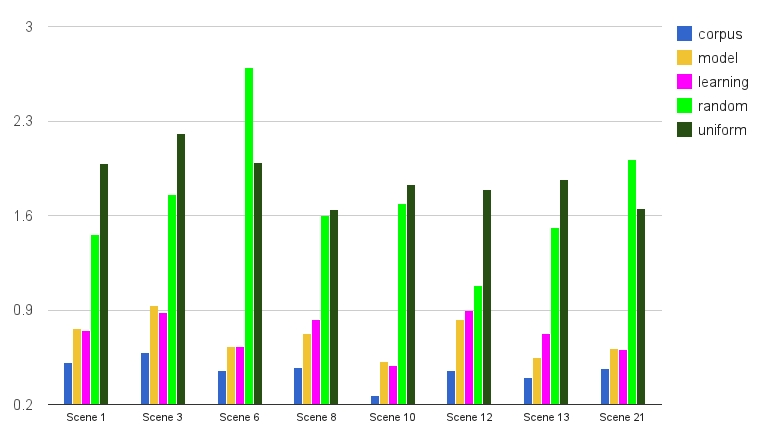
\includegraphics[width=.9\textwidth]{images/entropy.jpg}
\end{center}
\vspace*{-2em}
\caption{Cross-entropy between the corpus distribution of REs and each algorithm}\label{Entropy}
\end{figure}

In the figure we can observe that the learning and model cross-entropies are, in general, much closer to the corpus entropy than the random and uniform cross-entropies. Fig 12 is the only exception, where the random distribution is close to the learning and model because the randomly selected values of \puse are close to the learned values of \puse by chance. This exception is also evident in Table~\ref{results-algo-all} where random is 57.09\% for Fig 12.
In the figure we can also observe that the algorithm that uses the \puse directly calculated on the corpus of the scene (model) has a cross-entropy with respect to the corpus distribution that is very close to the cross-entropy between the corpus distribution and the distribution obtained by the algorithm when run with the \puse learned from corpora that does not describe the target scene (learning). This observation supports the learning mechanism proposed in Section~\ref{subsec:learning} to estimate the \puse when no corpora of REs of the target scene is available. 
